\section{Intermezzo}
\label{sec:intermezzo}

\begin{frame}
	\frametitle{Intermezzo: Algorithms to live by}
	\begin{columns}
		\column{0.455\textwidth}
	\begin{center}
		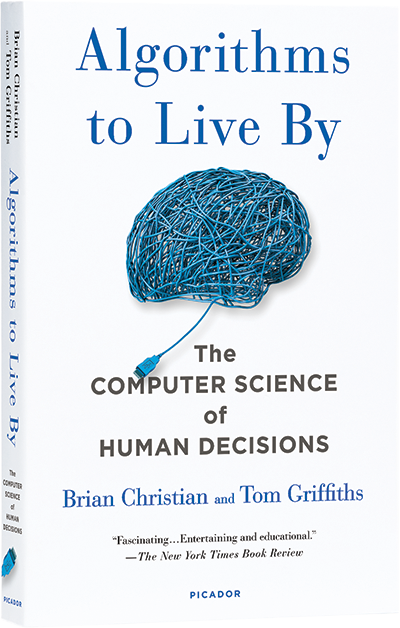
\includegraphics[width=0.6\textwidth]{figures/algorithms-to-live-by.png}\\
		\hspace*{15pt}\hbox{\scriptsize Image from \url{http://algorithmstoliveby.com/}}
	\end{center}
		\column{0.455\textwidth}
		\begin{itemize}
			\item I will give you few (outright) book recommendations this course.
				\pause
			\item But this one, you really should read :)
		\end{itemize}
	\end{columns}
\end{frame}

\begin{frame}
	\frametitle{The topics}
	\begin{itemize}
		\item Optimal Stopping: When are you not going to see better?
			\pause
		\item Explore/Exploit: When you should settle into a routine?
			\pause
		\item Sorting: Ah we know this one :) Includes bubble, insertion, merge and quicksort.
			\pause
		\item Caching: Includes notions of FIFO. What should we remember and what should we write down?
			\pause
		\item Scheduling: how do we handle deadlines?
			\pause
		\item Bayes' rule: Why probability is hard.
			\pause
		\item Overfitting, aka KISS (Keep It Simple Stupid)
			\pause
		\item Relaxation: a bit on NP-hard problems
			\pause
		\item Randomness: why do random decisions sometimes work out well?
			\pause
		\item Networking: issues in both Computer and Social networks.
			\pause
		\item Game Theory: Among other things, the prisoners' dilemma.
	\end{itemize}
\end{frame}

\begin{frame}
	\frametitle{Just one quote to wrap this up}
	
	\begin{quote}
		Some of the biggest challenges faced by computers and human minds alike: how to manage finite space, finite time, limited attention, unknown unknowns, incomplete information, and an unforeseeable future; how to do so with grace and confidence; and how to do so in a community with others who are all simultaneously trying to do the same
	\end{quote}
	By Brian Christian, Algorithms to Live By: The Computer Science of Human Decisions. As reported by Goodreads at:
	\url{https://www.goodreads.com/work/quotes/45489188}
\end{frame}


